\documentclass[a4paper,12pt]{article}
\usepackage{CodeReport}

\begin{document}


\begin{center} % Everything within the center environment is centered.
	{\Large \bf Coding Report 1} % <---- Don't forget to put in the right number
	\vspace{2mm}
	
       
	{\bf January 10, 2023}
\end{center}  

\vspace{0.4cm}


\section{Problem Description}

\section{Results}

\begin{figure}[H]
    \centering
	\begin{subfigure}[b]{0.49\textwidth}
	    \centering
	    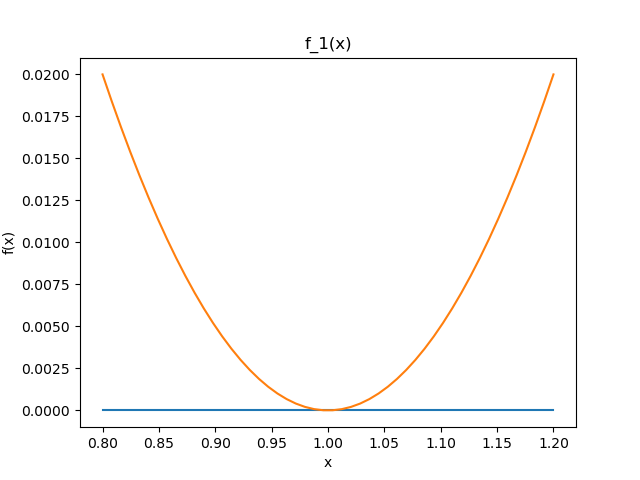
\includegraphics[width=\textwidth]{img/report1/f1.png}
	    \caption{$f_1(x) = \frac{1}{2}\sin((x - 1)^2)$}
	    \label{fig:0}
	\end{subfigure}
	\hfill
	\begin{subfigure}[b]{0.49\textwidth}
	    \centering
	     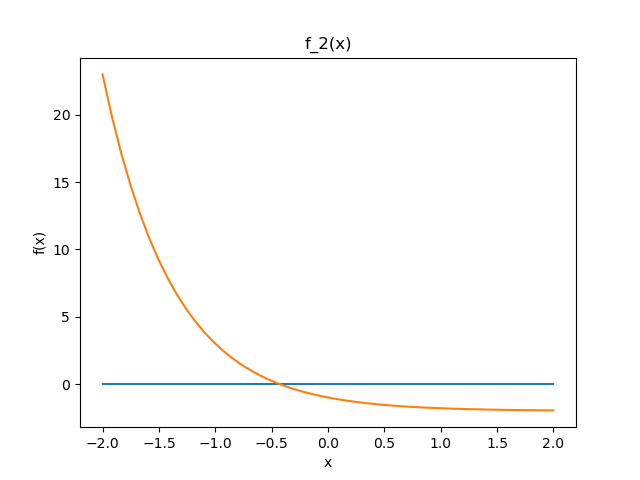
\includegraphics[width=\textwidth]{img/report1/f2.png}
	     \caption{$f_2(x) = 5^{-x} - 2$}
	     \label{fig:1}
	\end{subfigure}
\end{figure}



\begin{figure}[H]
	\begin{subfigure}[b]{0.49\textwidth}
	    \centering
	     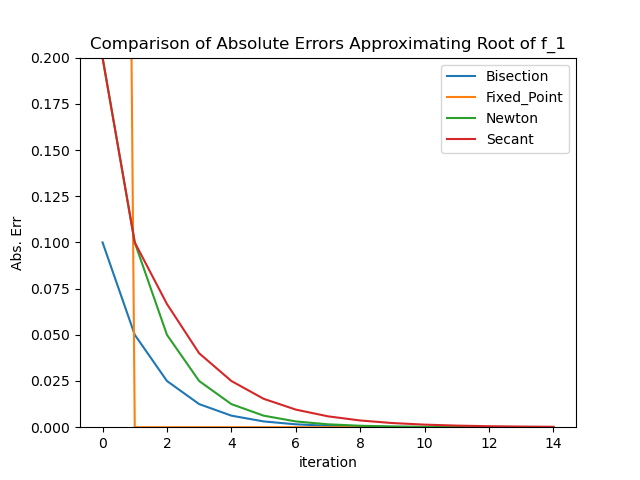
\includegraphics[width=\textwidth]{img/report1/f1_err.png}
	     \caption{Absolute Error of each methods approximating $f_1$ with respect to iteration.}
	     \label{fig:2}   
	\end{subfigure}
	\hfill	
	\begin{subfigure}[b]{0.49\textwidth}
	    \centering
	     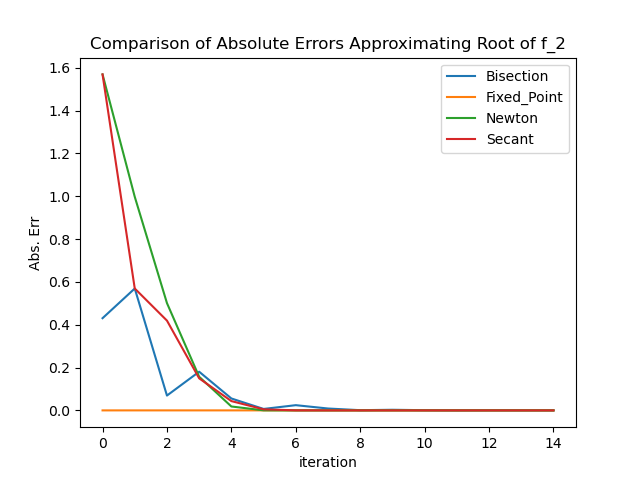
\includegraphics[width=\textwidth]{img/report1/f2_err.png}
	     \caption{Absolute Error of each methods approximating $f_2$ with respect to iteration.}
	     \label{fig:3}   
	\end{subfigure}
\end{figure}





\section{Collaboration}
No collaboration on this project.


\section{Academic Integrity}
On my personal integrity as a student and member of the UCD community, I have not given nor received any unauthorized assistance on this assignment.


\section{Appendix}

\lstinputlisting[language=Python]{numerical_methods/root_finding_1_var.py}
\lstinputlisting[language=Python]{report1.py}

\end{document}